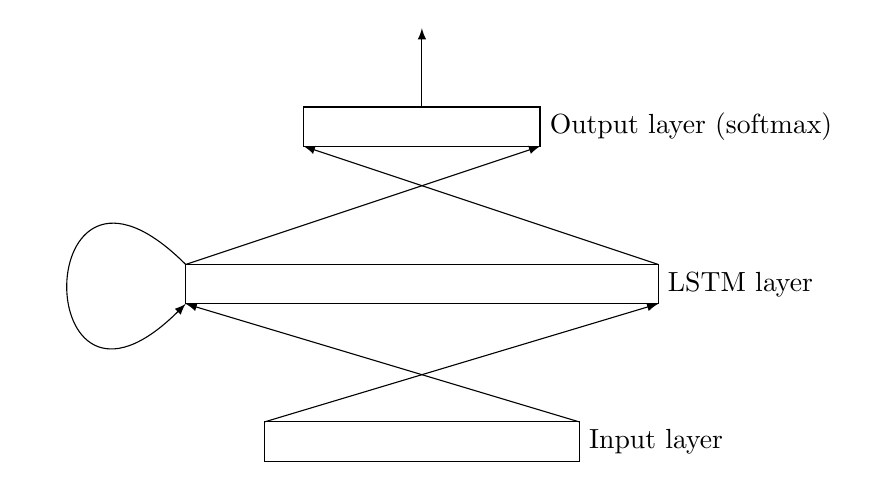
\begin{tikzpicture}
	\draw  (0,0) -- ++(2, 0) -- ++(0, 0.5) coordinate  (a)  node [midway, anchor=west] {Input layer} -- ++(-4, 0) coordinate  (b) -- ++(0, -0.5) -- cycle;
	
	
	\draw  (0,2) -- ++(3, 0) coordinate  (c) -- ++(0, 0.5) coordinate (d) node [midway, anchor=west] {LSTM layer}  -- ++(-6, 0) coordinate  (e) -- ++(0, -0.5)  coordinate  (f)  -- cycle;
	
	\draw  (0,4) -- ++(1.5, 0)  coordinate  (g) -- ++(0, 0.5) node [midway, anchor=west] {Output layer (softmax)}  -- ++(-3, 0) coordinate[midway] (t) -- ++(0, -0.5) coordinate  (h) -- cycle;	
	
	\draw[-latex] (a) -- (f);
	\draw[-latex] (b) -- (c);
	
	\draw[-latex] (e) -- (g);
	\draw[-latex] (d) -- (h);	
	
	\draw[-latex] (t) -- ++(0, 1);		
	\draw[-latex] (e)  .. controls ++(-2,2) and ++(-2, -2) ..  (f);
\end{tikzpicture}